
\documentclass[english]{article}
\usepackage{graphicx}
\usepackage{amsmath}
\usepackage{hyperref}
\usepackage{setspace}
\usepackage{apacite}
\usepackage{hyperref}
\usepackage{natbib}
\usepackage{pxfonts}
\usepackage[utf8]{inputenc}
\usepackage[left=1in,right=1in,top=1in,bottom=1in]{geometry}
\usepackage[left]{lineno}
\usepackage{soul}
\usepackage{setspace,caption}
\doublespacing
\captionsetup[figure]{labelsep=period,labelfont=it,justification=justified,
 singlelinecheck=false,font=doublespacing}
\usepackage[left=1in,right=1in,top=1in,bottom=1in]{geometry}
\linenumbers

\newcommand{\gazeLocations}{S1}
\newcommand{\excludedTrials}{S2}
\newcommand{\ratingsByCategory}{S3}
\newcommand{\sequenceLength}{S4}
\newcommand{\responseBias}{S5}

\begin{document}


\title{Category-based and location-based volitional covert attention affect
memory at different timescales}

\author{Kirsten Ziman$^1, 2$,
Madeline R. Lee$^1$,
Alejandro R. Martinez$^1$,\\
Ethan D. Adner$^1$,
and
Jeremy R. Manning\textsuperscript{$1, \dagger$}\\[0.1in]$^1$Dartmouth College\\
$^2$Princeton University\\
\textsuperscript{$\dagger$}Address correspondence to jeremy.r.manning@dartmouth.edu}

\maketitle

\begin{abstract} 
  
Our ongoing subjective experiences, and our memories of those experiences, are
shaped by our prior experiences, goals, and situational understanding. These
factors shape how we allocate our attentional resources over different aspects
of our ongoing experiences. These attentional shifts may happen overtly (e.g.,
when we change where we are looking) or covertly (e.g., without any explicit
physical manifestation). Additionally, we may attend to what is happening at a
specific spatial location (e.g., because we think something important is
happening there) or we may attend to particular features irrespective of their
locations (e.g., when we search for a friend's face in a crowd versus a
location on a map). We ran a covert attention experiment with two conditions
that differed in how long they asked participants to maintain the focus of the
categories and locations they were attending. Later, the participants performed
a recognition memory task for attended, unattended, and novel stimuli.
Participants were able to shift the location of their covert attentional focus
more rapidly than they were able to shift their focus of covert attention to
stimulus categories, and the effects of location-based attention on memory were
longer-lasting than the effects of category-based attention.

\noindent\textbf{Keywords: covert attention, spatial attention, category-based
attention, recognition memory, perception}

\end{abstract}


\section*{Introduction} 

Our brains' cognitive systems detect and exploit patterns in our prior and
ongoing experiences, enabling us to function and adapt in an ever-changing
world. However we do not attend to or treat all types of remembered or incoming
information equally, and our ability to flexibly adapt our thinking and
behaviors can vary markedly with the specific set of concepts or tasks relevant
to a given setting or situation~\citep{ChunTurk07, AlyTurk17, HardNade09,
RangRitc12}. There is also substantial variability across people with respect
to which aspects of experience (sensory, social, emotional, etc.) are noticed,
discriminated between, and acted upon~\citep{HuntEtal89}. This implies that the
same physical (objective) experience may give rise to very different perceived
(subjective) experiences across people~\citep{FreeSimo11, ChanEtal21a}.

The aspects of our experience we attend may be under our volitional control or
may be unconscious or automatic~\citep{JacoEtal92}. Both volitional and
unconscious attention may be expressed overtly, for example through intentional
eye movements~\citep{HoffSubr95} or covertly, without any volitional physical
change~\citep{EngbKlie03}. Prior work has explored the similarities and
differences in the neural basis of overt versus covert
attention~\citep{PosnEtal87, HuntKing03} as well as the behavioral and neural
underpinnings of volitional versus unconscious attention~\citep{DijkAart10} and
their differential effects on memory. There is a general consensus that
sustained volitional attention enhances memory relative to unconscious
attentional processes~\citep{UncaEtal11, TurkEtal13}. However, volitional
attention takes many forms, such as attention to particular spatial locations
or attention to particular visual features or other stimulus properties. How
different \textit{types} of volitional attention combine (or compete) to
enhance memory remains an open question. Volitional covert attention is of
particular interest in that it allows us to dynamically and intentionally
manipulate our experience, even when our sensory input remains largely
static~\citep[i.e., constant physical stimuli, retinal image, etc.][]{YiEtal06,
OcraEtal99}.

Here we examine the ways different types of volitional covert attention
interact to affect memory. We designed an experimental
paradigm~\citep[following][]{Posn80} that asked participants to attend to a
series of presented composite image pairs while keeping their gaze fixed on a
central point. The image pairs comprised a left and right image, each
constructed by blending an image of a face and place. The stimuli and
presentation durations were constant across the two experiments, but the
experiments differed in how often we asked participants to change the focus of
their attention with respect to image category (face versus place) and image
location (left versus right). After the participants attended to a series of
images, we used a recognition memory test to assess which aspects of the
presented images had been encoded into memory. In both experiments we found
that the images participants covertly attended to were better recognized than
other images, supporting the notion that attention enhances memory
encoding~\citep[i.e., they rated attended images as more familiar than
unattended images][]{Yone02}. After maintaining the focus of attention to a
single image category and location (Sustained Attention Experiment),
participants also recognized the attended-category image at the unattended
location, and (to a lesser extent) the unattended-category image at the
attended location. After more rapidly varying their focus of attention
(Variable Attention Experiment), participants showed a similar boost in
recognition for the unattended-category image at the attended location, but
they did not recognize images at the unattended location. This suggests that
participants were able to shift the location of their covert attentional focus
more rapidly than they were able to shift their focus of covert attention to
stimulus features. We also found differences in the timecourses of these memory
effects, suggesting that the impact of location-based attention on memory
persists on the order of several seconds longer than the impact of
feature-based attention.

\section*{Materials and methods}

We ran a total of 53 participants in across two experimental conditions
(Fig.~\ref{fig:paradigm}). The two conditions differed in how often we
cued participants to change the focus of their attention. All code and
documentation pertaining to our experiments and analyses, along with the
experimental stimuli and data, may be downloaded from
\url{http://www.github.com/ContextLab/attention-memory-task}.

\begin{figure*}[tp]
  \centering
  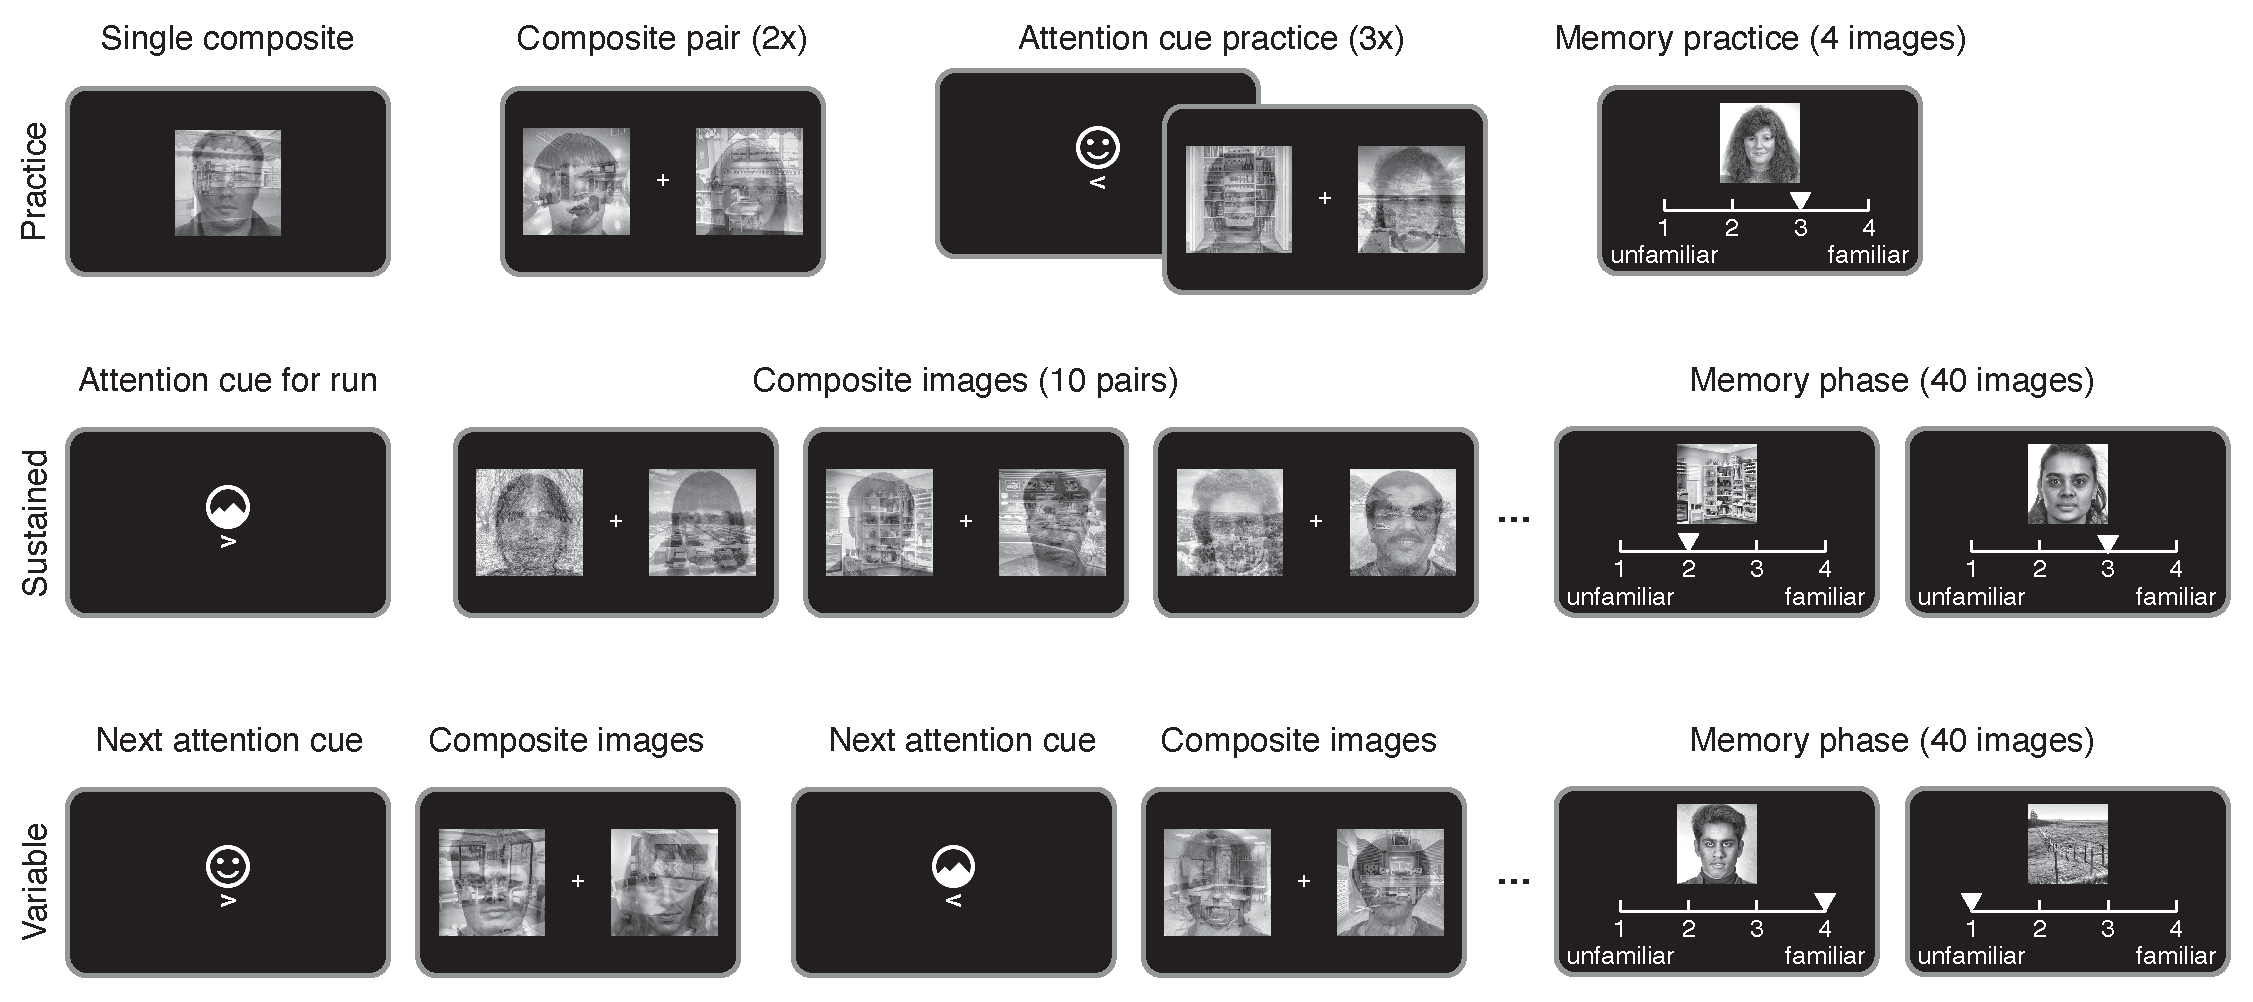
\includegraphics[width=1\textwidth]{figs/paradigm}

  \caption{\textbf{Experimental paradigm.} \textbf{A.--D. Practice phase.}
  \textbf{A.} Composite face/place image. \textbf{B.} A single pair of
  composite images and a central fixation cross. \textbf{C.} One attention cue
  practice trial. \textbf{D.} Familiarity judgement practice trial. \textbf{E.
  Sustained attention condition.} Participants receive an attention cue,
  followed by a sequence of 10 composite image pairs (Panel E), and then they
  make of familiarity judgements on each of 40 face and place images, presented
  in sequence (Panel F).  \textbf{G.  Variable attention condition.}  Participants
  study a succession of 10 composite image pairs, each preceded by an attention cue.
  After studying the images, they make a series of 40 familiarity judgements about
  face and place images, as in the sustained attention condition (Panel F).}

\label{fig:paradigm}
\end{figure*}

\subsection*{Participants} 

A total of 53 Dartmouth College undergraduate students enrolled in our study
(30 in the sustained attention condition and 23 in the variable attention
condition). Following a pilot study using a similar experimental design, we
aimed to enroll 30 participants in each condition. However, we fell short of
our enrollment target in the variable attention condition when in-person
testing was discontinued at our institution due to the COVID-19 pandemic. All
participants had self-reported normal or corrected-to-normal vision, memory,
and attention. Participants gave written consent to enroll in the study under a
protocol approved by the Committee for the Protection of Human Subjects at
Dartmouth College.

We used a voluntary pre-experimental survey to collect self-reported
demographic information about each partipant. All 53 participants elected to
fill out the survey. Participants ranged in age from 18--21 years old (mean:
18.7 years; standard deviation: 0.8 years). Participants reported their genders
as female (34 particiapnts), male (18 participants), and gender non-binary (1
participant). Participants reported their ethnicities as Not Hispanic or Latino
(44 particiapnts), Hispanic or Latino (7 participants), or declined to respond
(2 participant). Participants reported their race as White (37 participants),
Asian (13 participants), American Indian or Alaska Native (4 participants),
Black or African American (2 participants), and Other (1 participant). Note
that each participant could report one or more racial categories, as they
deemed appropriate.

Fourty-nine participants reported having no reading impairments, and 4
participants reported having reading impairments such as dyslexia. Fifty
participants reported having normal color vision and 3 reported having abnormal
color vision such as colorblindness. Fifty participants reported taking no
medications and having no recent injuries. One participant reported that they
had recently ``hit [their] head very hard.'' Another reported having taken
concerta in the past, but mentioned they had not taken it recently. One
participant reported using amphetamines regularly, but also clarified that they
were not currently on amphetamines at the time of testing.

We also asked participants to self-report on their sleep, alertness, and coffee
consumption. Participants reported having gotten between 4 and 9 hours of sleep
on the night prior to testing (mean: 6.9 hours; standard deviation: 1.3 hours).
Participants reported their alertness at the time of testing, and we converted
their responses to point values as follows: ``Very alert'' (5 points), ``A
little alert'' (4 points), ``Neutral'' (3 points), ``A little sluggish'' (2
points), and ``Very sluggish'' (1 point). Across all participants, the full
range of alertness values were used (maximum: 5; minimum: 1; mean: 3.44;
standard deviation: 1.0). Participants reported having consumed between 0 and 2
cups of coffee so far on their testing day (mean: 0.3 cups; standard deviation:
0.5 cups).

\subsection*{Stimulus selection and presentation} 

Participants viewed photographs of faces, places, and composite images each
comprising an equal blend of one face image and one place image. The pool of
360 face images included photographs of adult human male and female faces
selected from the FERET database~\citep{PhilEtal98}. The pool of 360 place
images included photographs of indoor and outdoor places selected from the SUN
database~\citep{XiaoEtal10}. The images we used from both databases came from a
stimulus subset that was manually curated by Megan deBettencourt (personal
communication). All images were resized to $256 \times 256$ pixels, converted
to greyscale, and processed so that every image was matched for mean contrast
and intensity. We selected 20 face images and 20 place images from the stimulus
pool to use in the instructional and practice phases of the experiments
(Fig.~\ref{fig:paradigm}A--D).

In addition to the face and place images, we presented (in white) attention
cues to direct the participant's focus of attention. The attention cues
comprised a stylized icon of a face or mountain peaks, directing attention to
the face or place component of the images, respectively; and a left- or
right-facing angled bracket, directing attention to the left or right image,
respectively (e.g., Figs.~\ref{fig:paradigm}C, E, and G).

 Our experiment was conducted in a sound- and light-attenuated testing room
 containing a chair, desk, and 27-inch iMac desktop computer (display
 resolution: $2048 \times 1152$). The participant sat in the chair and rested
 their chin on a chin rest located 60~cm from the display. The active portion
 of the display screen occupied 52.96$^\circ$ (width) and 31.28$^\circ$
 (height) of the participant's field of view from the chin rest. Stimuli were
 sized to occupy $6.7^\circ$ (width and height) of the participant's field of
 view from the chin rest. We maintained a black background (with any text
 displayed in white) throughout the experiment.

\subsection*{Eyetracking}

We recorded participants' eye gaze positions using a desk-mounted video-based
eyetracker with a spatial resolution of 0.1$^\circ$ visual angle root mean
squared error and a sampling rate of 30~Hz (Eye Tribe, The Eye Tribe,
Copenhagen, Denmark). We calibrated the eyetracker using a 9-point gaze
pattern. As described below, we re-calibrated the eyetracker at regular
intervals throughout the experiment to protect against camera drift.

We used the eyetracking data to home in specifically on behavioral effects
related to \textit{covert} attention, as opposed to overt looking effects.
Specifically, we excluded from further analysis any images from trials where
participants shifted their gaze (for any non-zero amount of time) to any part
of the attended composite image during a presentation trial
(see Figs.~\gazeLocations,~and \excludedTrials).

\subsection*{Experimental paradigm}

Our experiment comprised two testing conditions: a \textit{sustained} attention
condition and a \textit{variable} attention condition. Both experimental
conditions comprised a practice phase followed by a series of eight task
blocks. Each task block was in turn comprised of a presentation phase and a
memory phase. The practice and presentation phases differed across the two
experiments, and the memory phases were identical across the two experiments.
Both experiments were implemented using PsychoPy~\citep{PeirEtal19}.

\subsubsection*{Practice phase}

Several participants in pilot versions of our experiments reported that they
found it difficult to modulate the focus of their attention quickly on command.
We therefore designed a practice sequence to orient the participant to the
process of quickly modulating the focus of their attention without moving their
eyes. The experimenter remained in the testing room throughout the practice
phase and answered any questions about the experiment. The practice sequence
builds up incrementally to provide a gradual on-ramping for the participant
prior to beginning the main experimental tasks that we focused on in our
analyses.

\paragraph{Practice shifting the focus of category-based attention to elements
of a single composite image.}

At the start of the practice phase, we instructed the participant to look at a
single composite (face-place blend) image at the center of the screen, and to
try to bring the face component of the image into greater focus by attending to
it (Fig.~\ref{fig:paradigm}A). After pressing a button on the keyboard to
indicate that they had done so, we displayed a second composite image and
instructed the participant to bring the place component of the new composite
image into focus. Again, they pressed a button to indicate that they had done
so.

\paragraph{Practice shifting the focus of category-based and location-based
attention while viewing two composite images.}

Next, we asked the participant to stare at a fixation cross presented in the
center of the screen while two composite images were displayed on the left and
right side of the screen, respectively (Fig.~\ref{fig:paradigm}B). We first
instructed the participant to attend to the place component of the left image
without moving their eyes. Participants practiced shifting their attention, and
they pressed a button on the keyboard to indicate that they had done so. We
then displayed a second pair of composite images and instructed the participant
to attend to the face component of the right image. Again, the participant
shifted their attention in a self-paced manner, and pressed a button to
indicate when they had successfully done so.

\paragraph{Practice \textit{sustaining} category-based and location-based attention over
a series of composite image pairs.}

We asked participants in the sustained attention condition to practice holding
their focus of category-based and location-based attention constant (to the
face component of the right image) while viewing a series of three composite
image pairs presented in succession (Fig.~\ref{fig:paradigm}C).

\paragraph{Practice \textit{varying} category-based and location-based
attention over a series of composite image pairs.}

We asked participants in the variable attention condition to practice varying
their focus of category-based and location-based attention while viewing a
series of three composite image pairs, each presented after a different
attention cue (Fig.~\ref{fig:paradigm}C).

\paragraph{Practice reaction time probe.}

After practicing modulating their focus of attention to a series of composite
image pairs, we introduced a reaction time probe after each image presentation,
whereby we presented either an $\times$ or $\circ$ on either the left or the
right of the screen (not shown). We asked the participant to press the
\texttt{1} key as quickly as possible when they saw an $\times$, or the
\texttt{3} key as quickly as possible when they saw an $\circ$. We did not
impose a time limit on their responses, other than asking participants to
respond as quickly as they were able. Participants practiced three trials of
modulating their focus of attention to a pair of composite images (3~s), and
reacting as quickly as possible to the $\times$ or $\circ$ symbol presented
after each composite image pair. The reaction time probe was intended to keep
participants continually engaged in modulating the focus of their attention.

\paragraph{Practice recognition memory task.}

Finally, we asked the participant to practice reporting familiarity on a
recognition memory task (Fig.~\ref{fig:paradigm}D). We presented a single face
or place image at the center of the screen, and asked them to press a button to
indicate how ``familiar'' the image seemed: \texttt{1} (very confident they had
not seen the image), \texttt{2} (somewhat confident they had not seen the
image), \texttt{3} (somewhat confident they had seen the image), or \texttt{4}
(very confident that they had seen the image). We instructed the participant to
go with their ``gut reaction'' in the event that they were unsure of how to
respond. We allowed the participant up to 2~s to provide their response. We
gave participants a total of four practice images to rate.

After completing the practice phase of the experiment, the participant read the
instructions for the task blocks (described next). The experimenter gave
participants a chance to ask any remaining questions about the experiment.
After answering the participant's questions, the experimenter calibrated the
eyetracker and exited the testing room.

\subsubsection*{Task blocks}

During each task block we asked the participant to modulate their attention
while viewing a series of 10 composite image pairs (each followed by a reaction
time probe), and then we tested the participant's memory using 40 familiarity
judgements. Each participant completed a total of eight task blocks.

\paragraph*{Sustained attention condition: presentation phase
(Fig.~\ref{fig:paradigm}E).}

Participants viewed an attention cue (1.5~s) instructing them to attend to
either the face or place component of either the left or right images in each
to-be-viewed composite pair. Next we displayed 10 composite images in
succession (each preceded by a fixation cross and proceeded by a reaction time
probe). All possible attention cue pairs appeared exactly twice across the
eight task blocks.

\paragraph*{Variable attention condition: presentation phase
(Fig.~\ref{fig:paradigm}G).}

Participants viewed a succession of 10 attention cues (1.5~s), each followed by
a fixation cross (1~s), composite image (3~s), and a reaction time probe. The
attention cues were selected pseudorandomly across trials within each block,
with the constraints that no single attention cue pair could appear more than
three times across the 10 composite image pairs within a single task block.

\paragraph*{Memory phase (Fig.~\ref{fig:paradigm}F).}

After the presentation phase of each task block, we asked the participant to
rate the familiarity (on a 1--4 scale, as during the practice phase) of a
succession of face and place images. Each image was preceded by a 1~s fixation
cross, and participants had up to 2~s to input their rating of each image.
Participants made a total of 40 familiarity judgements, about 20 face images
and 20 place images. Of these, 20 of the images (10 faces and 10 places) were
drawn randomly from the (attended and unattended) composite images that the
participant had viewed during the presentation phase. The remaining 20 images
(10 faces and 10 places) were novel images that the participant had not
encountered during any part of the experiment. At the end of each memory block,
the participant was given the opportunity to take a short break. When they were
ready to continue with the next task block, they indicated their readiness to
the experimenter. The experimenter then entered the testing room, re-ran the
eyetracker calibration sequence, and exited the testing room prior to the next
task block.

\section*{Results}

We ran a volitional covert attention experiment with two conditions; in the
sustained attention condition we asked participants to \textit{sustain} the
focus of their attention over a succession of 10 stimulus presentations per
block whereas in the variable attention condition we asked participants to
\textit{vary} their focus of attention with each new stimulus (also for a total
of 10 stimulus presentations per block). Each stimulus comprised a pair of
composite images (one on the left and one on the right side of the display),
where each composite comprised an equal blend of a unique face and a unique
place image. We followed the presentation phases of each experimental block
with a memory phase, where participants performed a recognition memory task by
rating the familiarity of previously experienced and novel face and place
images (see \textit{Experimental paradigm}, Fig.~\ref{fig:paradigm}).

\begin{figure*}[tp]
	\centering
	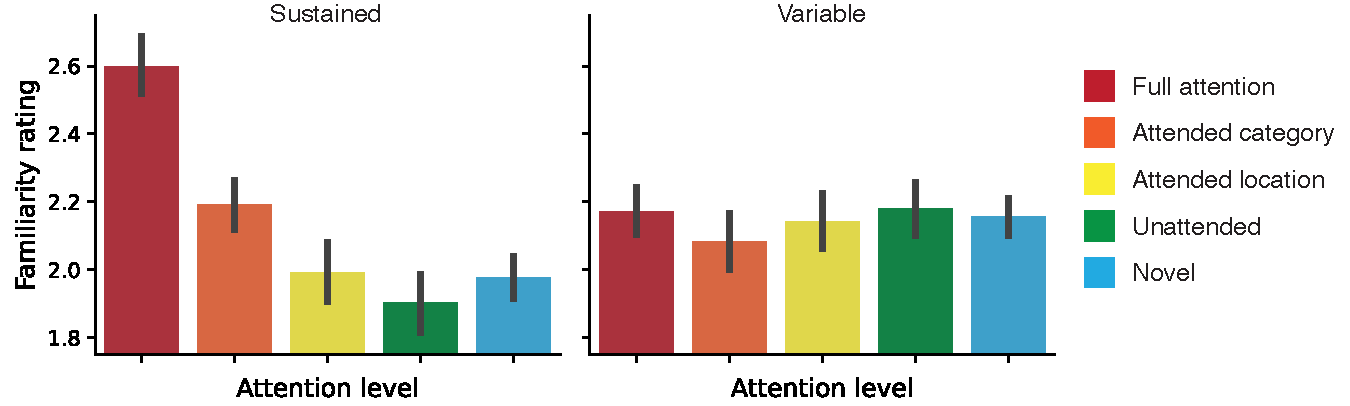
\includegraphics[width=0.7\textwidth]{figs/familiarity_by_attention_level}
  
  \caption{\textbf{Familiarity by attention level.} The bars display the
  average familiarity ratings participants gave to images from the same
  category and location as the attention cue (fully attended), the same
  category (but opposite location) as the attention cue (attended category),
  the same location (but opposite category) as the attention cue (attended
  location), the opposite category and location as the attention cue
  (unattended), or novel images. The left panel displays familiarity ratings
  from the sustained attention condition and the right panel displays
  familiarity ratings from the variable attention condition. All error bars
  denote across-participant bootstrap-estimated 95\% confidence intervals. For results
  sub-divided by stimulus category, see Figure~\ratingsByCategory.}
  
  \label{fig:familiarity}
  \end{figure*}

We first wondered whether (and how) shifts in covert attention might affect
participants' ratings during the recognition memory task
(Fig.~\ref{fig:familiarity}). To ensure that our findings were not conflated
with where people were physically looking, we excluded from further analysis
any images presented during trials where the participant's gaze touched on any
part of the attended composite image (see \textit{Eyetraciking},
Figs.~\gazeLocations~and \excludedTrials). For the remaining trials, the
participants kept their gaze focused on a fixation cross at the center of the
screen while \textit{covertly} shifting the focus of their attention to the
cued category component of the composite image on the cued location. In other
words, during these remaining trials, participants' physical (external)
experiences of the face and place components of every presented composite image
remained relatively constant across trials (up to our ability to accurately
measure where participants were looking using the eyetracker). 

Simply by encoding their prior experiences into memory, we reasoned that
participants should rate \textit{any} presented images as more familiar than
novel images, regardless of whether they were following the attention cues. We
confirmed that this prediction held in both the sustained ($t(29) = 8.856, p <
0.001$) and variable ($t(22) = 5.144, p < 0.001$) conditions. In addition, to
the extent that participants were following the attention cues, there
\textit{internal} experiences of each image should depend on their internal
focus of attention during each image presentation. For example, we expected
that the attended-category component of the composite image at the attended
location might be better recognized than the other composite image components.
Indeed, participants in both experimental conditions rated these ``fully
attended'' images as more familiar than category-matched image components from
unattended locations (sustained: $t(29) = 6.893, p < 0.001$; variable: $t(22) =
6.938, p < 0.001$), location-matched images from the unattended category
(sustained: $t(29) = 6.710, p < 0.001$; variable: $t(22) = 7.633, p < 0.001$),
unattended images that were neither from the attended category nor the attended
location (sustained: $t(29) = 8.470, p < 0.001$; variable: $t(22) = 7.256, p <
0.001$), or novel images they had never seen before (sustained: $t(29) =
10.259, p < 0.001$; variable: $t(22) = 7.874, p < 0.001$).

We also wondered whether the ways participants attended to or remembered the
images might depend on image-specific properties like the images' categories.
We repeated the analyis displayed in Figure~\ref{fig:familiarity} separately
for face and place images (Fig.~\ratingsByCategory). The same general patterns
held for each category, as when we combined across the two stimulus categories
as reported above. For example, fully attended face and place images were both
rated as more familiar than the category-matched images from the unattended
location (sustained: $t$s$(29) \geq 3.36, p$s$ \leq 0.002$; variable: $t$s$(22)
\geq 6.205, p$s$ \leq 0.001$), attended-location images from the unattended
category (sustained: $t$s$(29) \geq 5.886, p$s$ \leq 0.001$; variable:
$t$s$(29) \geq 4.277, p$s$ \leq 0.001$), images from the unattended category
and location (sustained: $t$s$(29) \geq 6.628, p$s$ \leq 0.001$; variable:
$t$s$(29) \geq 5.624, p$s$ \leq 0.001$), and novel images (sustained: $t$s$(29)
\geq 5.987, p$s$ \leq 0.001$; variable: $t$s$(29) \geq 5.132, p$s$ \leq
0.001$). Taken together, the above results suggest that what we remember is
guided in part by what we attended to, even after accounting for where we look
or what specifically we are looking at.

Splitting participants' responses to face versus place images also revealted
that participants often rated attended (and partially attended) place images as
more familiar than attention-matched face images (compare dark versus light
bars in Fig.~\ratingsByCategory). We hypothesized that this might be
explainable by some property of the relevant cognitive processes or by
properties of the stimuli themselves. To help elucidate this distinction, we
examined individual exemplars of the face and place images used in our paradigm
(Fig.~\ref{fig:stimuli}A). By design, the face images had consistent head
sizes, viewing angles, expressions, and so on. In contrast, the place images
varied more substantially across images. For example, some place images
depicted human-made structures; others depicted natural scenes; some depicted
indoor views; others depicted outdoor views; etc. This can also be seen by
averaging the pixel intensity values across images, separately for the face and
place stimuli (Fig.~\ref{fig:stimuli}B). Whereas the average face image retains
many of the landmarks characteristic of most faces (e.g., clearly defined hair,
eyes, nose, mouth, head shape, etc.), the average place image does not show
place-specific features as clearly, aside from a general tendancy for the tops
of place images to be lighter than the bottoms of place images. We also
computed the pairwise similarities across images from each stimulus category
(Fig.~\ref{fig:stimuli}C) and found that face images tended to be much more
similar to each other than place images (Fig.~\ref{fig:stimuli}D; $t(115258) =
254.764, p < 0.001$). This analysis indicated to us that our experimental
paradigm was not well-suited to identifying cognitively meaningful stimulus
category differences, since participants' category-specific judgements may be
confounded with within-category image similarity differences.


\begin{figure*}[tp]
	\centering
	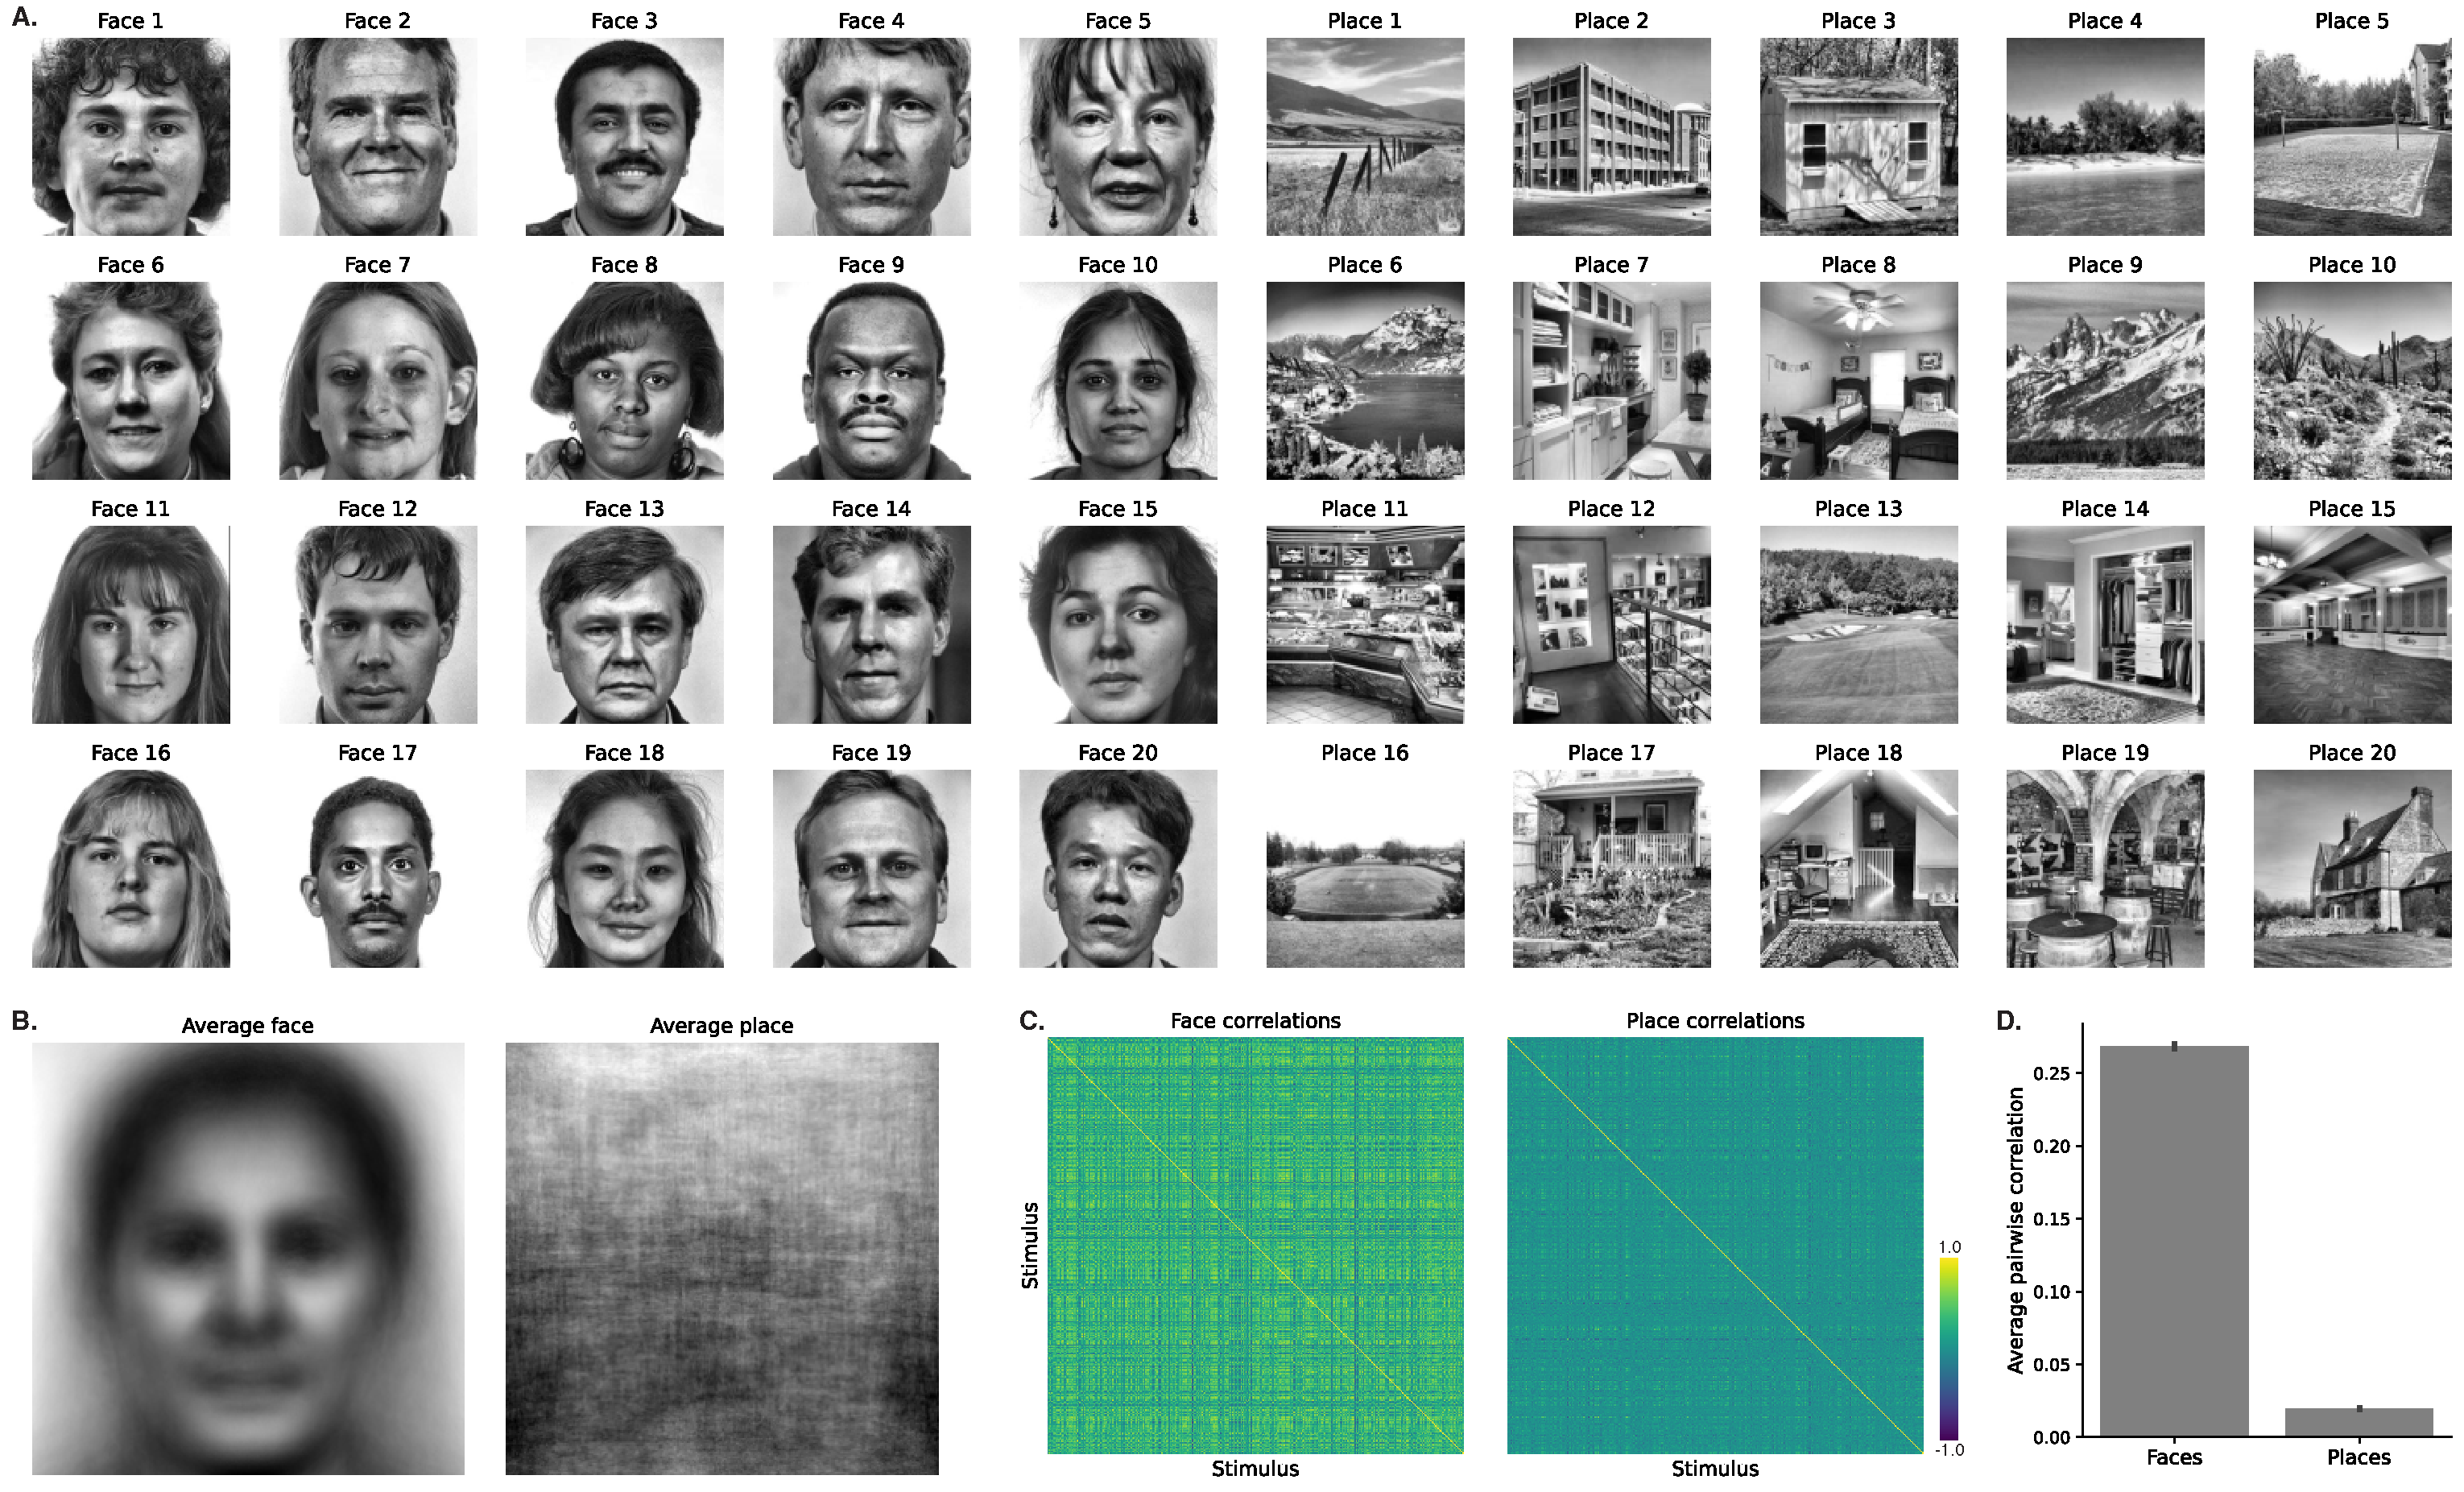
\includegraphics[width=\textwidth]{figs/stimuli}
  
  \caption{\textbf{Stimulus examples and properties.} \textbf{A. Example images
  from each stimulus category.} Randomly chosen subsets of 20 face images
  (left) and 20 place images (right) are displayed. \textbf{B. Across-image
  averages.} Each panel displays the average image, taken across all 360 face
  images (left) and 360 place images (right). \textbf{C. Pairwise
  correlations.} Each row and column of the matrices displays the correlation
  (across pixels) in intensity values for one pair of face images (left) or
  place images (right). \textbf{D. Average pairwise correlations.} The bar
  heights denote the average pairwise correlations between face and place
  images. Error bars denote across-pair bootstrap-estimated 95\%
  confidence intervals.}
  
  \label{fig:stimuli}
  \end{figure*}

Next, we turned to identifying potential differences in participants' behaviors
across the two experimental conditions. The main difference between the
conditions' procedures was in how long participants were asked to maintain the
same focus of category-based and location-based attention, across successive
image presentations. Therefore, differences in participants' behaviors across
the two conditions might reflect differences in the timescales of the relevant
cognitive processes. We compared participants' familiarity ratings for images
at each attention level across the two conditions. We saw no evidence that
people rated fully attended images ($t(51) = -0.649, p = 0.519$),
attended-category (but not location) images ($t(51) = 1.163, p = 0.250$), or
novel images ($t(51) = -0.435, p = 0.665$) differently across the two
conditions. However, participants in the variable attention condition rated
attended-location (but unattended category) images as more familiar than
participants in the sustained attention condition ($t(51) = 2.174, p = 0.034$).
We found a trending effect for unattended category and location images, whereby
participants in the variable attention condition tended to rate these images as
more familiar than participants in the sustained attention condition ($t(51) =
1.600, p = 0.116$). We also observed some within-condition differences in how
participants rated partially attended versus novel images. In the sustained
attention condition, participants rated attended-category images at the
unattended location as more familiar than novel images ($t(29) = 6.205, p <
0.001$), but participants in the variable attention condition did not show this
pattern ($t(22) = 1.042, p = 0.309$). On the other hand, whereas participants
in the sustained attention condition showed no reliable differences in
familiarity between attended-location images from the unattended category and
novel images ($t(29) = 0.165, p = 0.870$), participants in the variable
attention condition rated attended-location images as more familiar than novel
images ($t(22) = 3.026, p = 0.006$). Taken together, our analyses highlight
several familiarity differences in partially attended images from the attended
category or at the attended location across the two experimental conditions.
These differences suggest that category-based versus location-based attention
operate over different timescales.

\begin{figure*}[tp]
	\centering
	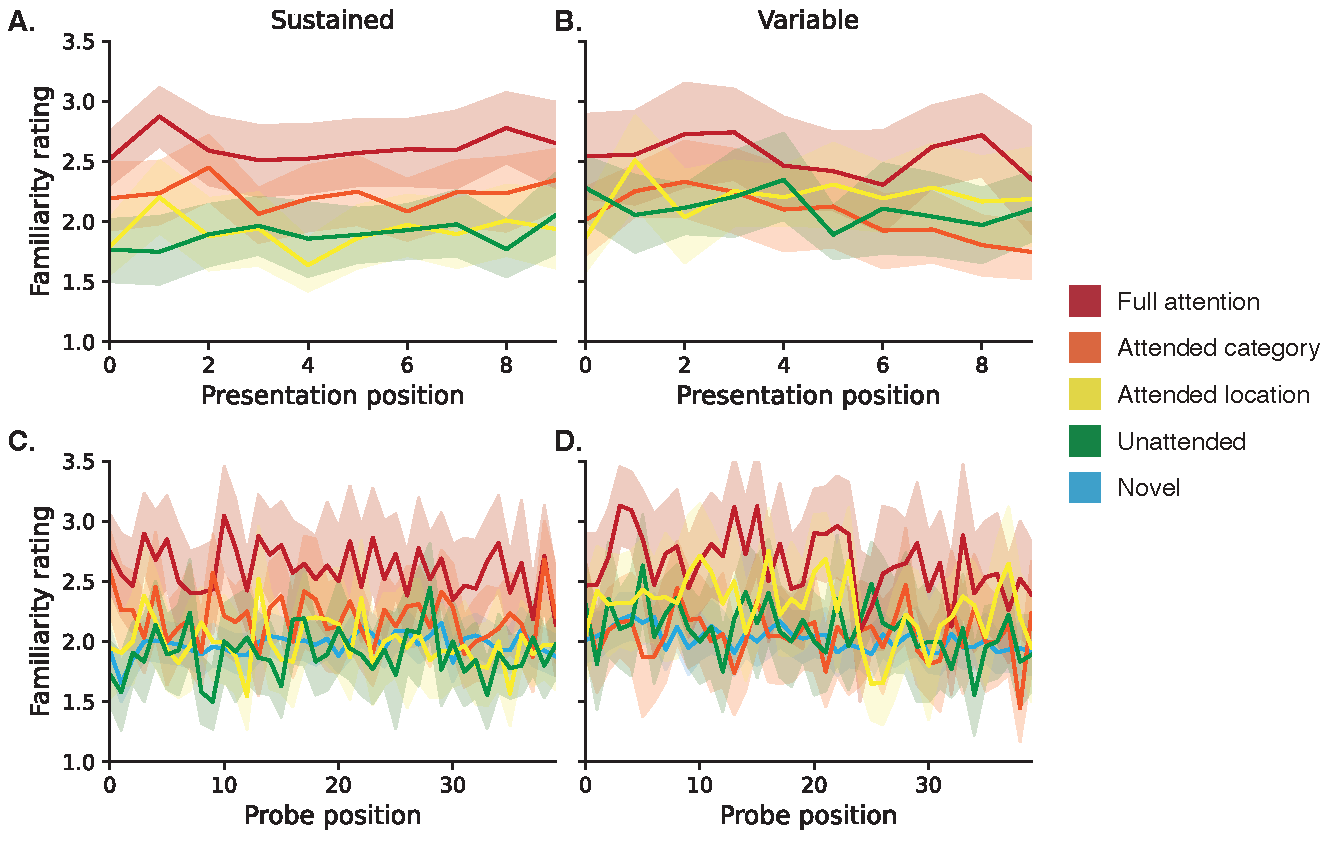
\includegraphics[width=0.7\textwidth]{figs/encoding_and_retrieval_timecourses}
  
  \caption{\textbf{Familiarity ratings by serial positions and attention
  level.} \textbf{A. Subsequent familiarity ratings by presentation position
  (sustained attention condition).} The curves' colors denote the attention
  levels of each presented image. The $x$-axis denotes the presentation
  positions of each image within the sequence of 10 composite image pairs
  during the run when it was presented. The $y$-axis denotes the average
  familiarity ratings later given to the corresponding items. \textbf{B.
  Subsequent familiarity ratings by presentation position (variable attention
  condition).} This panel is in the same format as Panel A, but displays
  ratings for the variable attention condition. \textbf{C. Familiarity ratings
  by memory probe position (sustained attention condition).} The curve's colors
  denote the attention levels (or novelty) of each probe image. The $x$-axis
  denotes the position of each probed image within the sequence of 40 images
  that participants judged during the memory phase of the experiemnt. The
  $y$-axis denotes the average familiarity ratings given to the corresponding
  probes. \textbf{D. Familiarity ratings by memory probe position (variable
  attention condition).} This panel is in the same format as Panel C, but
  displays ratings for the variable attention condition. All panels: error
  ribbons denote across-participant bootstrap-estimated 95\% confidence
  intervals.}
  
  \label{fig:timecourses}
  \end{figure*}

Given the above results suggesting potential differences in the timescales of
category-based and location-based attention, we carried out two additional
exploratory analyses aimed at identifying other timing effects. First, we
wondered whether participants' familiarity ratings might show serial position
effects analogous to those reported in classic recognition memory
studies~\citep[e.g.,][]{Neat93b, McElDosh89, WickNorm66}. For each participant,
for each composite image pair (presented in each trial during the study phase
of the experiment), we labeled each composite's face and place image component
according to whether it matched the cued category and/or location. We discarded
any face or place images that did not appear in the participants' memory phase.
We tagged the remaining (probed) images with the familiarity ratings that
participants would later give the images during the memory phase and plotted
these ratings against the images' presentation positions
(Figs.~\ref{fig:timecourses}A and B). Across both experimental conditions and
across all serial positions, we generally found that the average ordering of
familiarity ratings by attention level (Fig.~\ref{fig:familiarity}) were
preserved. This suggests that the encoding-related affects of attention on
subsequent recognition memory are relatively stable over time (e.g., we did not
observe clear primacy or recency effects during the study phase of the
experiment). Second, we carried out an analogous analysis to identify potential
serial position effects of recall order. For each probed item a participant
rated during the memory phase, we assigned the image a label according to
whether the participant's attention cue (at the time the image was presented as
part of its composite pair) matched the image's category and/or location, or
whether the image was novel (i.e., not presented during the study phase).
Again, we found that (across both experimental conditions and all probe
positions) in general the average ordering of familiarity ratings by attention
level (Fig.~\ref{fig:familiarity}) were preserved. This suggests that the
retrieval-related affects of attention on subsequent recognition memory are
relatively stable over time (e.g., we did not observe clear primacy or recency
effects during the memory phase of the experiment).

Our finding that location-attended items appear to receive a familiarity boost
in the variable attention condition but not the sustained attention condition
is consistent with two possible interpretations. One possibility is that
focusing attention requires just a brief trigger (in this case, an attention
cue), but different forms of attention (in this case, category-based attention
versus location-based attention) require different amounts of time to ``ramp
up'' to full efficacy such that they begin to affect memory encoding. For
example, if category-based attention ramps up more slowly than location-based
attention, this might explain why the relative ordering of category-matched
versus location-matched unattended images changes between the sustained
attention and variable attention conditions (orange and yellow bars in
Fig.~\ref{fig:familiarity}). A second possibility is that each attention cue
provides a ``boost'' to memory encoding for the relevant aspects of one's
experience (e.g., image categories, spatial locations), but the size of the
boost varies across different forms of attention. If so, the \textit{number} of
successive attention cues one receives should predict how effectively the
attended and partially attended images are encoded. We developed a sequence
length analysis to distinguish between these possibilities. For each probed
(target) image that had been presented as a composite image pair, we computed
the number of matching attention cues the participant had received by the time
the given images were presented (up to and including the image's composite
pair). We computed these sequence lengths by defining ``matching'' cues in
three ways: (a) a match means the cues are for the same category \textit{and}
location, (b) a match means that the cues are for the same category, and (c) a
match means that the cues are for the same location. This yielded, for each
target image, an associated count of how many matching attention cues the
participant had received up to and including that image's presentation. As
shown in Figure~\sequenceLength, we used linear regressions of familiarity
rating on sequence lengths to identify potential sequence length effects. For
both experimental conditions, all attention levels, and for all three
approaches to defining matching cue sequence lengths, we found virtually no
reliable associations between cue sequence length and familiarity. This finding
is most parsimonious with the first possiblity mentioned above-- i.e., that
attention may be guided by a brief trigger, but that different forms of
attention may take differently long to affect memory encoding.

Finally, we wondered whether participants' familiarity ratings might be
influenced in part by response bias effects. For example, a participant who had
recently received an ``attend to face images'' cue might rate a probed face
images as more ``familiar'' even if they had no specific memories for the given
image. Indeed, participants in the sustained attention condition do show some
response biases. For example, participants tended to rate novel images as more
familiar if they came from the just-cued category (Fig.~\responseBias A; $t(29)
= 4.371, p < 0.001$). Responses biases are more difficult to evaluate in the
variable attention condition. For example, should cue recency be defined as the
number studied composite image pairs that came between the image whose
familiarity the participant is judging and the most recent save-category cue
(i.e., distance to the nearest same-category probe)? Or might response biases
instead arise when a given category is cued more often near the end of the
just-studied list? We assigned each probed image a label based on these two
measures of category-matched cue recency. We then used linear regressions of
familiarity on these recency measures to identify potential response biases
(Fig.~\responseBias B). Altogether we found no evidence that participants in
the variable attention condition tended to rate images as more familiar solely
due to how recently they had received a same-category attention cue.

\section*{Discussion}

We ran a covert attention experiment with two conditions that asked
participants to sustain or vary the focus of their covert attention,
respectively. We then administered recognition memory tests that asked
participants to rate the ``familiarity'' of attended, unattended, and novel
images. In our analyses, we used eyetracking data to focus in on trials where
participants were specifically varying their focus of \textit{covert} attention
(i.e., with no change in external behavior), as opposed to simply moving their
eyes to look at the to-be-attended images. In both conditions, we found that
participants recognized images from the attended category and location more
readily than unattended or novel images. This effect was substantial and robust
(in both conditions) and also held for individual image categories. Whereas
prior work has focused primarily on \textit{overt} changes in attention (e.g.,
changes in eye movements associated with attention cues), we show that what
people \textit{covertly} attend to also affects how they remember their ongoing
experiences.  Specifically, covert attention appears to boost memory encoding
such that the focus of covert attention is recognized more readily later on.

\begin{figure*}[tp]
  \centering \includegraphics[width=0.75\textwidth]{figs/discussion_schematic}

  \caption{\textbf{How do covert location-based and category-based attention
  affect memory encoding?}\textbf{A. Hypothesized timecourses of the impact of
  location-based and category-based attention on memory encoding.} Shifting the
  focus of location-based attention increases memory encoding at the attended
  locations (blue curve). This increase can be observed after 5.5~s (the
  duration of one presentation from the variable attention condition). Shifting
  the focus of category-based attention suppresses memory encoding for the
  unattended category. However, this suppression effect occurs relatively
  slowly (longer than the duration of a single image presentation in the
  experiment). \textbf{B. Location-based attention.} Focusing covert attention
  on one \textit{location} enhances encoding of stimuli at the attended
  location (red and yellow bars), regardless of stimulus category.  (This panel
  is based on the variable attention results presented in Fig.~\ref{fig:familiarity}.)
  \textbf{C. Category-based attention.}  Focusing covert attention on one \textit{category}
  supresses encoding of stimuli from the unattended category (yellow and green bars),
  regardless of spatial location.  (This panel is based on the sustained attention
  results presented in Fig.~\ref{fig:familiarity}.)}

\label{fig:discussion}
\end{figure*}

We also found that partially attended images (e.g., from the attended category
but unattended location, or at the attended location but unattended category)
were rated as more familiar than novel images. However, these encoding benefits
differed across the two experimental conditions. In the sustained attention
condition, attended-category images from the unattended location were rated as
more familiar than novel images, but attended-location images from the
unattended category were not. Participants in the variable attention condition
showed the opposite pattern. The variable attention participants rated
attended-\textit{location} images from the unattended category as more familiar
than novel images, but they rated attended-category images from the unattended
location similarly to novel images. Because the primary difference between the
sustained and variable attention conditions was the duration of the attention
cues, our analyses of partially attended images suggest that the effects of
different aspects of attention on memory may unfold over different timescales
(Fig.~\ref{fig:discussion}). Specifically, location-based attention appears to
affect memory encoding relatively quickly, which would explain why
attended-location images from both the attended \textit{and} unattended
category receive a memory encoding benefit in the variable attention condition.
In contrast, category-based attention appears to affect memory encoding more
slowly, and it appears to operate in a ``suppressive'' manner (i.e., supressing
encoding of the unattended category, as opposed to enhancing encoding of the
attended category). This would explain why unattended-category images at the
attended location are rated as \textit{less} familiar in the sustained
attention condition.

\textbf{JRM STOPPED HERE}

When participants held the focus of their category-based (face
versus place) and location-based (left versus right) attention for a sustained
interval, they judged stimuli they had seen as familiar when they overlapped
with respect to the features and locations they had attended. The increase in
familiarity was larger for attended-feature images than attended-location
images. The increase also extended to novel stimuli from the attended image
category. By contrast, when participants varied the focus of their
feature-based and location-based attention more rapidly, the boost in
familiarity for feature-matched stimuli was smaller than that for
location-matched stimuli, and did not extend to novel stimuli. Our findings
suggest that participants were able to more rapidly modulate their focus of
location-based attention than their focus of feature-based attention. The
tuning of location-based attention appears to be mediated by enhanced encoding
and faster processing at the attended location. The tuning of feature-based
attention appears to be mediated by a suppression in the encoding and
processing of unattended stimulus features. This suppression effect also
affects how new stimuli are processed, and it persists for a longer duration
following an interval when the focus of feature-based attention was held
constant over a longer duration. Taken together, our findings suggest that
feature-based and location-based attention are mediated by different mechanisms
and affect memory at different timescales (Fig.~\ref{fig:model}).

% \begin{figure*}[tp]
%   \centering \includegraphics[width=0.75\textwidth]{figures/discussion_schematic}

%   \caption{\textbf{Timecourse of encoding and retrieval effects of
%   feature-based and location-based attention.} The focus of location-based
%   attention (green) may be modulated quickly and rapidly enhances memory
%   encoding for nearby stimuli. The focus of feature-based attention (purple) is
%   modulated more slowly, and serves to suppress unattended stimulus features.
%   The effects of location-based attention on memory persist for longer than the
%   effects of feature-based attention. Sustained attention (darker shading)
%   yields more robust enhancement and suppression than shorter-term (variable)
%   attention (light shading). The vertical gray line on the left denotes the
%   duration of a single stimulus presentation (the upper bound by which
%   location-based attention begins to affect encoding, and the lower-bound by
%   which feature-based attention begins to affect encoding). The vertical gray
%   line on the right separates encoding from immediate subsequent retrieval of
%   the encoded information.}

% \label{fig:model}
% \end{figure*}

The notion that location-based attention operates at a faster timescale than
feature-based attention is supported by prior work on the deployment of visual
attention~\citep{SotoBlan04, StopEtal07}. Our findings that location-based
attention enhances the processing of attended stimuli whereas feature-based
attention suppresses the processing of unattended stimuli is also consistent
with prior work on location-based attention~\citep[e.g.,][]{IttiKoch01} and
feature-based attention~\citep[e.g.,][]{MoheEtal14}. Our finding that people
better remember attended stimuli also follows prior work on interactions
between attention and memory~\citep{PallWagn02, ChunTurk07, AlyTurk16,
AlyTurk17, WittEtal18, MorrEtal14, BaleEtal21}. Whereas much of this prior work
focused on elucidating the neural basis of these interactions, our work extends
these prior studies by elucidating the specific and separable behavioral
impacts of feature-based attention (inhibition with a slow onset) and
location-based attention (enhancement with a fast onset) on subsequent memory.
Both of these effects persisted throughout the 2~min memory phases of both
experiments. Therefore future work is needed to elucidate the longevity of
these effects beyond 2 minutes.

Another important area for future study concerns how the flow of information
between different brain structures is modulated according to the focus of
volitional attention-- particularly with respect to pathways from primary
sensory regions (e.g., V1, A1) to regions implicated in encoding ongoing
experiences into memory (e.g, medial temporal lobe structures such as the
hippocampus and entorhinal cortex, prefrontal cortex, etc.). For example,
several studies suggest that attention serves to modulate the \textit{gain} of
specific neural circuits~\citep{TreuTruj99, ChanEtal02, EldaEtal13,
SaliThie00}, effectively facilitating or inhibiting the flow of specific neural
representations~\citep{VartEtal07, LaRoEtal14}. Prior work suggests that
feature-based attention may be supported by changes in connectivity with the
thalamus~\citep{Schn11}, whereas location-based attention may be supported by
changes in connectivity with primary visual cortex~\citep{NoudEtal10}. That
feature-based and location-based attention are mediated by different brain
structures may explain why these different aspects of attention operate on
different timescales and affect memory differently. A strong test of this
hypothesis would entail directly measuring neural activity patterns as people
modulate their focus of attention (e.g., using functional magnetic resonance
imaging or electroencephalography), and then using neural decoding
approaches~\citep[e.g.,][]{HaxbEtal01, NormEtal06b, MannEtal18} to follow how
neural representations of attended (or unattended) stimuli are transfered from
primary sensory regions, to higher order sensory regions, to memory areas. If
the effects of attention on memory are mediated by changes in network dynamics,
the transmission rates of the representations of attended stimuli from primary
sensory regions to memory areas should be facilitated relative to the
transmission rates of unattended stimuli. Further, variability in these neural
changes (e.g., as a participant focuses their attention with more or less
success) should track with behavioral measures of memorability.

Which aspects of our ongoing experiences we choose to attend affects how we
process and remember those experiences later. Different forms of
attention---e.g., to specific features or spatial locations---operate and
affect memory at different timescales, and are likely mediated by different
brain networks. Elucidating the behavioral and neural consequences of
volitional changes in attention is central to discovering how our thoughts,
feelings, goals, and situational understanding fluctuate from moment to moment.


\section*{Author Contributions}

JRM and KZ developed the concept for this study. Experiment code was written by
KZ and ARM, and testing and data collection were conducted by MRL and KZ. KZ,
MRL, ARM, and JRM analyzed the data. JRM supervised the project. All authors
contributed to writing and editing the manuscript.

\section*{Data and code availability}

All of the data analyzed in this manuscript, along with all of the code for
running our experiment and carying out the analyses may be found at
\url{http://www.github.com/ContextLab/attention-memory-task}.


\section*{Acknowledgements}

This work was supported in part by NSF EPSCoR Award Number 1632738 to JRM and
by by NSF CAREER Award Number 2145172 to JRM. The content of this manuscript is
solely the responsibility of the authors and does not necessarily represent the
official views of our supporting organizations. We are grateful for useful
discussions with the EPSCoR Attention Consortium, particularly with Marian
Berryhill, Gideon Caplovitz, Patrick Cavanagh, Theresa Desrochers, and Peter
Tse. We thank Megan deBettencourt for useful discussions, pointers to our
experimental stimuli, and for providing code to facilitate stimulus
preparation. We also appreciate useful discussions with Paxton Fitzpatrick,
Kevin Hartstein, Talia Manning, Lucy Owen, and Michael Ziman. Finally, we thank
Christina Liu and Eowyn Pak for their help running pilot versions of the
experiments reported here.


\bibliographystyle{apacite}
\bibliography{CDL-bibliography/cdl}



\end{document}
